\begin{figure}[tbp]
\centering
\begin{tikzpicture}[x=.88cm,y=.88cm,font=\small,
 every node/.style={align=center},line cap=round,line join=round,
 row/.style={draw,circle,fill=white,inner sep=3pt}]
 \filldraw[fill=gray!7,draw=gray!60] (.1,3.7) rectangle (5.55,4.8);
 \filldraw[fill=gray!7,draw=gray!60] (6.45,3.7) rectangle (11.9,4.8);
 \node[font=\footnotesize] at (2.8,5.08) {replacement of $t^iH$};
 \node[font=\footnotesize] at (9.2,5.08) {replacement of $t^{i-1}H$};
 \node[row] (pm) at (.8,4.22) {$P_-$};
 \node[row] (q) at (2.8,4.22) {$Q$};
 \node[row] (pp) at (4.8,4.22) {$P_+$};
 \node[row] (pms) at (7.2,4.22) {$P_-$};
 \node[row] (qs) at (9.2,4.22) {$Q$};
 \node[row] (pps) at (11.2,4.22) {$P_+$};
 \draw (pm)--node[above] {$I$} (q);
 \draw (q)--node[above] {$J$} (pp);
 \draw[thick,dashed,orange!75!black]
   (pp)--node[above,font=\footnotesize] {shift} (pms);
 \draw (pms)--node[above] {$I$} (qs);
 \draw (qs)--node[above] {$J$} (pps);
 \draw[->,thick] (6,3.55)--(6,2.75);
 \node[anchor=west,font=\footnotesize] at (6.18,3.18)
   {collapse the shift edge};
 \node[row] (aq) at (2.8,2.15) {$Q$};
 \node[row] (ap) at (6,2.15) {$P$};
 \node[row] (aqs) at (9.2,2.15) {$Q$};
 \draw[densely dotted] (.9,2.15)--(aq);
 \draw (aq)--node[above] {$J$} (ap);
 \draw (ap)--node[above] {$I$} (aqs);
 \draw[densely dotted] (aqs)--(11.1,2.15);
 \node[below=7pt] at (aq.south) {$i$};
 \node[below=7pt] at (ap.south) {$i-\tfrac12$};
 \node[below=7pt] at (aqs.south) {$i-1$};
 \draw[->,gray!70!black] (8.2,.35)--(3.8,.35);
 \node[font=\footnotesize,fill=white] at (6,.35) {increasing height};
\end{tikzpicture}
\caption{A local part of the actual row refinement. Each coarse row is
replaced by $P_-*_{I}Q*_{J}P_+$. The original shift edge has
isomorphisms at its two $P$-endpoints and can be collapsed; the $I$-
and $J$-edges remain. The heights shown below agree with $h(t)=1$.
Each displayed group is in the actual conjugate frame of its coarse
row. The picture shows a local path, not the whole Bass--Serre tree;
the quotient by $L$ is a line, while the actual tree can branch.}
\label{fig:row-refinement}
\end{figure}
